\definecolor{ttqqcc}{rgb}{0.33,0.33,0.33}
%dash pattern=on 5pt off 2pt
%[fill = white, rounded corners = 4pt, inner sep = 1pt]
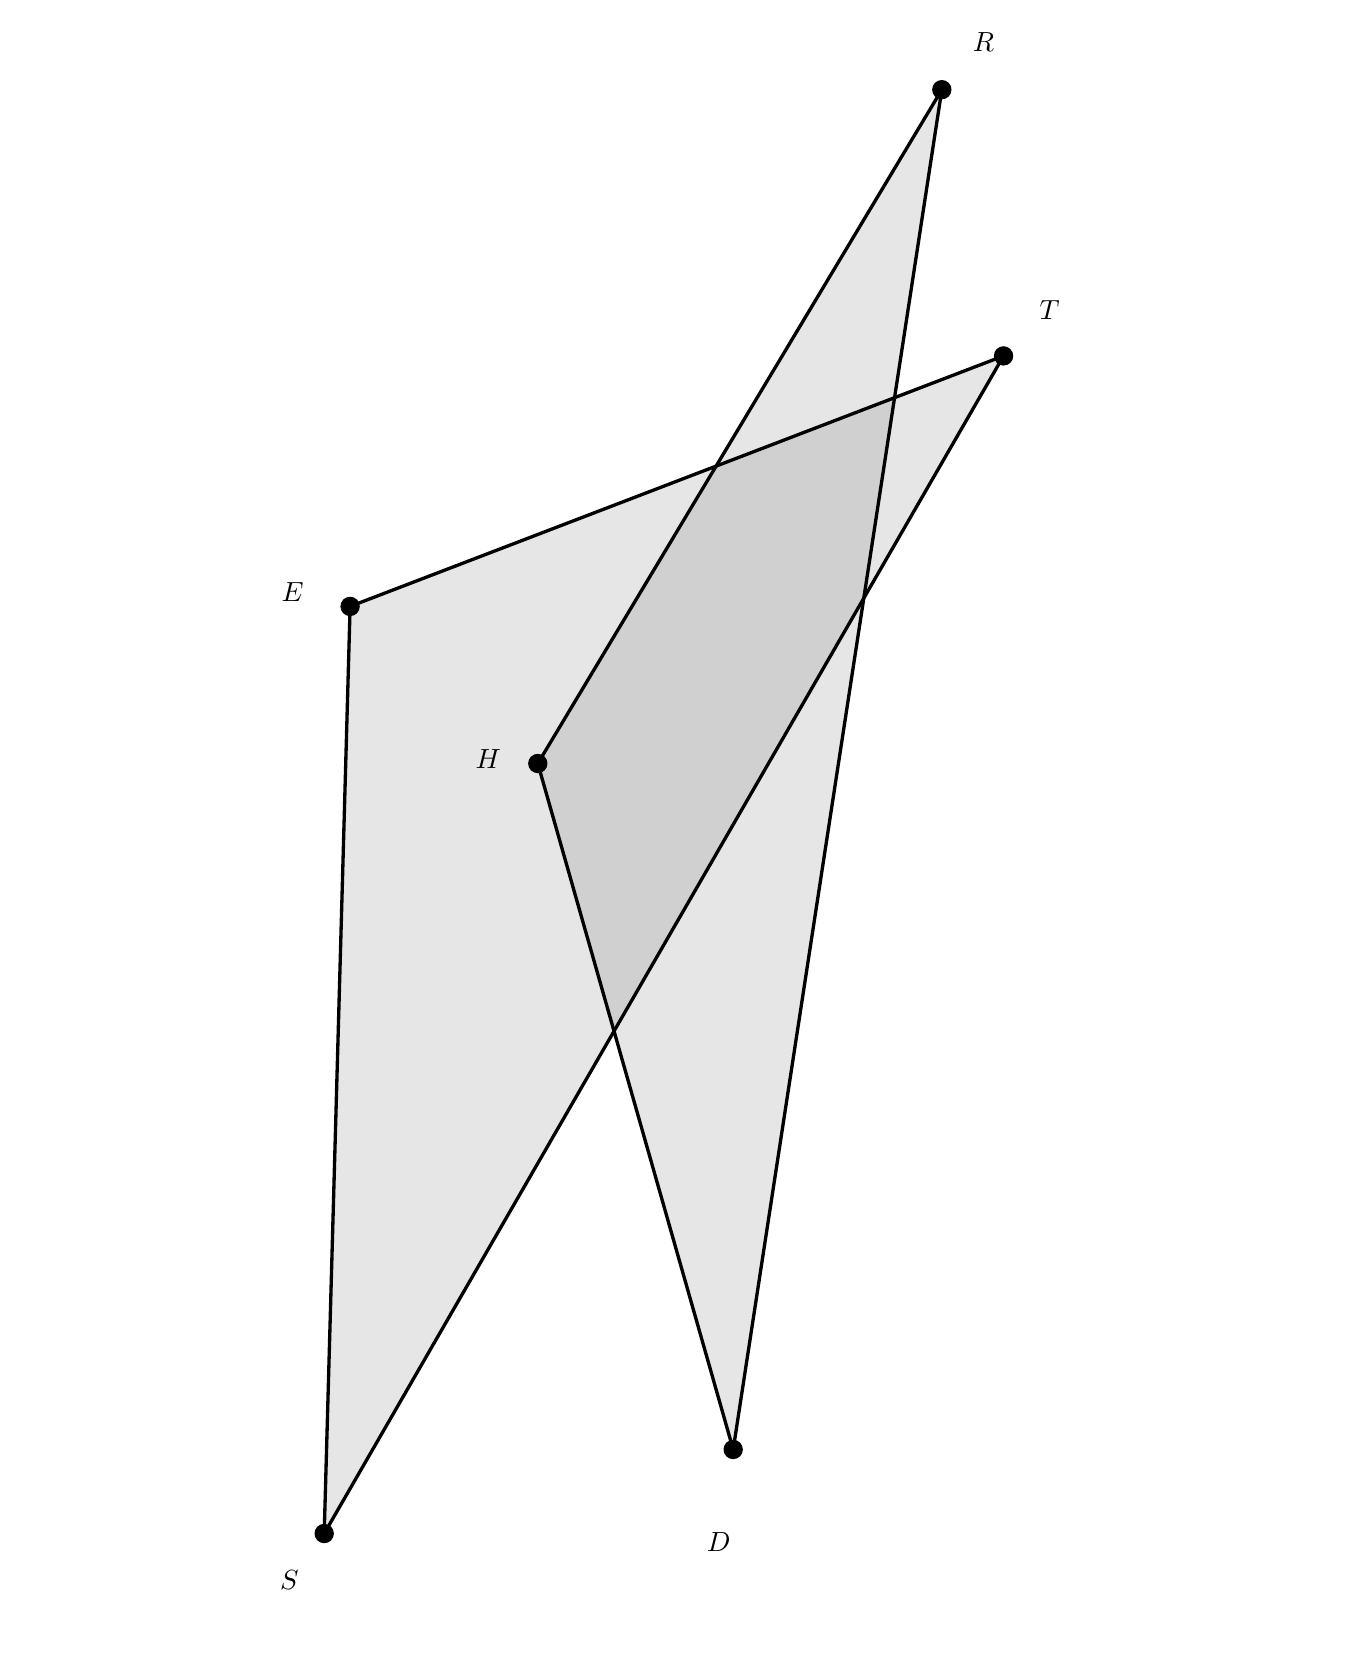
\begin{tikzpicture}[scale = 0.35]
    \clip(-25.62,-26.69) rectangle (21.49,31.61);
    \fill[line width=0pt,color=ttqqcc,fill=ttqqcc,fill opacity=0.15] (9.79,19.7) -- (-13.92,10.61) -- (-14.86,-23.03) -- cycle;
    \fill[line width=0pt,color=ttqqcc,fill=ttqqcc,fill opacity=0.15] (7.55,29.36) -- (-7.11,4.91) -- (-0.02,-19.98) -- cycle;
    \draw [line width=1.2pt] (9.79,19.7)-- (-13.92,10.61);
    \draw [line width=1.2pt] (-13.92,10.61)-- (-14.86,-23.03);
    \draw [line width=1.2pt] (-14.86,-23.03)-- (9.79,19.7);
    \draw [line width=1.2pt] (7.55,29.36)-- (-7.11,4.91);
    \draw [line width=1.2pt] (-7.11,4.91)-- (-0.02,-19.98);
    \draw [line width=1.2pt] (-0.02,-19.98)-- (7.55,29.36);
    \begin{scriptsize}
        \normalsize
        \fill [color=black] (-13.92,10.61) circle (10pt);
        \draw[color=black] (-16.01,11.13) node {$E$};
        \fill [color=black] (-14.86,-23.03) circle (10pt);
        \draw[color=black] (-16.12,-24.7) node {$S$};
        \fill [color=black] (9.79,19.7) circle (10pt);
        \draw[color=black] (11.46,21.37) node {$T$};
        \fill [color=black] (7.55,29.36) circle (10pt);
        \draw[color=black] (9.06,31.08) node {$R$};
        \fill [color=black] (-7.11,4.91) circle (10pt);
        \draw[color=black] (-8.91,5.07) node {$H$};
        \fill [color=black] (-0.02,-19.98) circle (10pt);
        \draw[color=black] (-0.55,-23.35) node {$D$};
    \end{scriptsize}
\end{tikzpicture}